\section{Review of the Bitcoin Peer-to-Peer Network}
Bitcoin is built on top of a peer-to-peer network. To connect to the network, a local client uses four main methods of bootstrapping to locate an initial remote node.  The first is the internal database of addresses the client saved during the previous session.  If none of those addresses are active or the client is being run for the first time, the client uses a hard-coded DNS service to locate the address of seed nodes.   The third method is via hard-coded addresses of seed nodes.  The final method uses user inputted addresses from the command line or loaded from a text file.  The Bitcoin network also previously used Internet Relay Chat (IRC) bootstrapping, but support for this method has been removed as of Bitcoin version 0.8.2.

To connect to a remote node, the client node first sends a {\tt Version} message to the remote node. If the remote node accepts the {\tt Version} message it replies with a {\tt Verack} message and its own {\tt Version} message. If the client node accepts the remote node's {\tt Version} message, it replies with a {\tt Verack} message.  Finally, both nodes exchange {\tt GetAddr} messages and {\tt Addr} messages, which include the node's address information as well as no more than 2,500 addresses seen in the last 3 hours in the node's internal address database.

\begin{figure}[ht!]
\begin{center}
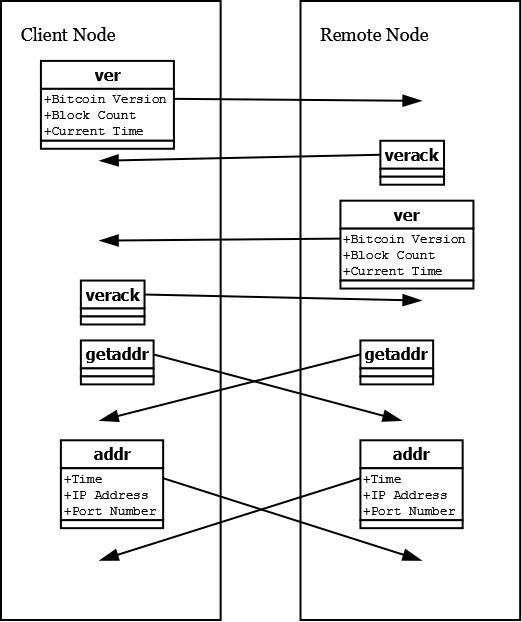
\includegraphics[scale=0.3]{./images/bitcoin_peer_protocol.png}
\caption{Bitcoin connection setup.}
\label{fig:bitcoin_peer_protocol}
\end{center}
\end{figure}

After a node has joined the Bitcoin P2P network, peer discovery is propagated by callback addresses, {\tt Addr} messages relays, and self broadcast. Callback addresses are addresses in the remote node's {\tt Version} message that enable the local node to connect back.  If the local node does connect back, then as described above, the local node will exchange {\tt Addr} messages.  Address relays occur after new addresses are added into the local node's internal database. The local node will pick two random nodes in its database and relay the new addresses in another {\tt Addr} message. A node will also self broadcast, in which the node advertises its own address in an {\tt Addr} message to all connected nodes.

\section{Boomerang Overview}
At its heart, Boomerang is a protocol to emulate a peer-to-peer mixnet that can be leveraged by any anonymizing coin, such as Zerocoin, to provide anonymity properties analogous to Tor without the same side channel vulnerabilities and need for an additional software component. The main idea is to hide the source or origin from which transactions are introduced into the network. To do this, we integrate traditional mixnet behavior into the peer-to-peer Bitcoin network so that new transactions which are to be broadcasted must first pass through a series of mixes (which are actually other participating Bitcoin users) in the network so as to obfuscate the originating network address. Functionally, this is not much different from Tor. However, Boomerang has several important distinctions that make it unique:
\begin{enumerate}
	\item Transaction anonymity increases \emph{for every participant} when more people use Boomerang messages to broadcast transactions - everyone is therefore incentivized to use Boomerang. 
	\item Involuntary mixing delays mitigate timing-based side channel attacks that can be leveraged to deanonymize clients using Tor. 
	\item Boomerang messages are enhancements to the Bitcoin protocol, rather than a means for anonymizing point-to-point TCP connections. 
\end{enumerate}

The main design goals of Boomerang are as follows:
\begin{description}
	\item[{\bf Sender anonymity}]: \\A node achieves \emph{sender anonymity} if a node cannot be (uniquely) identified, or linked, to a particular transaction that is broadcast at the end of a Boomerang circuit (see Section \ref{sec:design}) \cite{AnonymityTerms}. 
	\item[{\bf Fault-tolerance via redundancy}]: \\Compromised or mobile nodes should not lead to significant delays in transaction broadcasts or induce traffic deadlocks.
	\item[{\bf Performance}]: \\Nodes in the network should incur minimal overhead from using Boomerang messages while maximizing their anonymity.
\end{description}

We now provide a brief overview of how Boomerang is used by clients for transaction broadcast anonymity; A complete description of the protocol is provided in Section 4. To broadcast a new transaction $T$ using Boomerang, a client $C$ first creates a set of $W$ individual mixing circuits of length $D_1,D_2,\dots,D_W$, where $W \geq 1$ and $D_i \geq 2$. Let $K = \sum_{i=1}^WD_i$ be the total number of nodes selected as mixing services for the circuits. With knowledge of the public keys for each of the $K$ nodes, $C$ then wraps $T$ in $D_i$ layers of encryption for each circuit $i = 1,\dots,W$. Each layer of encryption also includes a forward pointer to the subsequent hop in the circuit so that decrypting nodes may forward the transaction to the appropriate location, or broadcast the plaintext transaction $T$ if they are the last hop in the circuit. 

As is standard with traditional mix networks, each nodes will only forward wrapped transactions after it has accumulated a certain number of transactions from other nodes \cite{Chaum81-Mix}. For this reason, to avoid network deadlock, we require that ``cover traffic'' be circulated throughout the network to keep traffic moving smoothly, similar to the cover traffic used in the Tarzan mix network \cite{tarzan}. Furthermore, this cover traffic must be encoded such that it appears indistinguishable from legitimate encrypted transaction messages. To solve this problem, Boomerang cover traffic messages \emph{are themselves legitimate transaction encryptions}, with the exception that the last hop of the circuit for these messages is the same client $C$ that generated them in the first place. Thus, these dummy transaction messages will be circulated throughout the network and ultimately routed back to $C$, who can then easily check that they generated the transaction and discard it (or send out another dummy message). The cyclical flow of cover traffic, which is shown by the red trajectories in Figure \ref{fig:boomerang_net}, is the inspiration for Boomerang's name.

\begin{figure}[ht!]
\begin{center}
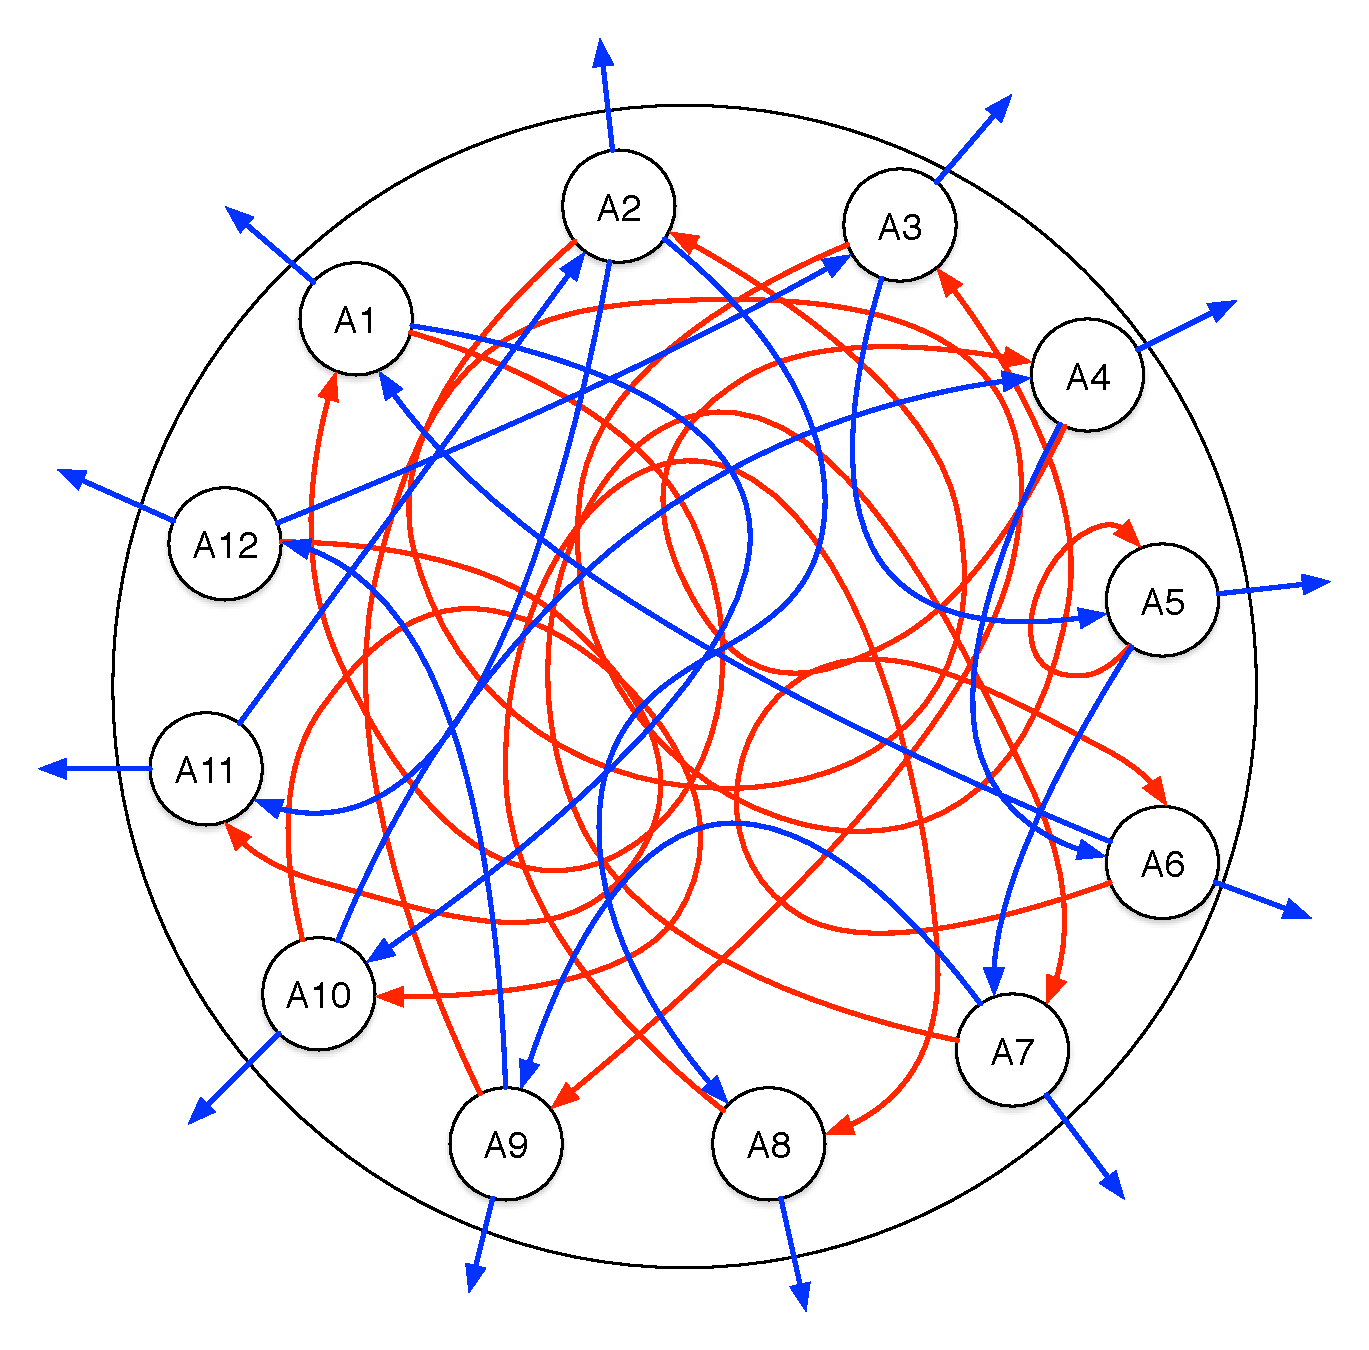
\includegraphics[scale=0.25]{./images/boomerang_net.pdf}
\caption{Visual depiction of the traffic flow in a Boomerang network.}
\label{fig:boomerang_net}
\end{center}
\end{figure}

Given this short description, there are many important engineering problems to solve in order make Boomerang feasible in practice, such as public key distribution and usage, prevention of self-induced denial-of-service, and an overconsumption of network resources. We describe solutions to all such problems in Section 4, and include a preliminary performance analysis of the Boomerang technique (based on analytical modeling and simulations) in Section 5. 
